
\begin{comment}
\begin{figure}[t]
  \centering
  \resizebox{\linewidth}{!}{%
    \begin{circuitikz}
      \path[use as bounding box] (0,-8.5) rectangle (18,19.5); % tighten bbox
      \tikzstyle{every node}=[font=\large]
\draw [ fill={rgb,255:red,224; green,237; blue,212} , line width=0.8pt , rounded corners = 9.0] (1.25,17.5) rectangle  node {\LARGE Caption} (3.75,16.25);
\draw [ fill={rgb,255:red,202; green,240; blue,254} , line width=0.8pt , rounded corners = 9.0] (0,15.5) rectangle (5,-3.25);
\node [font=\Large] at (2.5,15) {LLM};
\draw [line width=0.8pt, ->, >=Stealth] (2.5,16.25) -- (2.5,15.5);
\draw [ fill={rgb,255:red,224; green,237; blue,212} , line width=0.8pt ] (3.75,14.25) rectangle (4.25,13.75);
\draw [ fill={rgb,255:red,224; green,237; blue,212} , line width=0.8pt ] (0.75,14.25) rectangle (1.25,13.75);
\node [font=\Large] at (-3.5,12.75) {};
\node [font=\Large] at (-3.5,12.75) {};
\node [font=\Large] at (-4.25,12.75) {};
\draw [ fill={rgb,255:red,224; green,237; blue,212} , line width=0.8pt ] (1.75,14.25) rectangle (2.25,13.75);
\draw [ fill={rgb,255:red,224; green,237; blue,212} , line width=0.8pt ] (2.75,14.25) rectangle (3.25,13.75);
\draw [ fill={rgb,255:red,224; green,237; blue,212} , line width=0.8pt ] (0.25,13.25) rectangle  node {\large LLM Block} (4.75,12.75);
\draw [line width=0.8pt, ->, >=Stealth] (2.5,13.75) -- (2.5,13.25);
\node [font=\Huge] at (3,13) {};
\node [font=\Huge] at (3,13) {};
\node [font=\Huge] at (3,13) {};
\draw [line width=0.8pt, ->, >=Stealth] (2.5,12.75) -- (2.5,12.25);
\draw [ fill={rgb,255:red,224; green,237; blue,212} , line width=0.8pt ] (3.75,12.25) rectangle (4.25,11.75);
\draw [ fill={rgb,255:red,224; green,237; blue,212} , line width=0.8pt ] (0.75,12.25) rectangle (1.25,11.75);
\draw [ fill={rgb,255:red,224; green,237; blue,212} , line width=0.8pt ] (1.75,12.25) rectangle (2.25,11.75);
\draw [ fill={rgb,255:red,224; green,237; blue,212} , line width=0.8pt ] (2.75,12.25) rectangle (3.25,11.75);
\draw [ fill={rgb,255:red,224; green,237; blue,212} , line width=0.8pt ] (0.25,8.75) rectangle  node {\large LLM Block} (4.75,8.25);
\draw [line width=0.8pt, ->, >=Stealth] (2.5,11.5) -- (2.5,8.75);
\node [font=\Huge] at (3,8.5) {};
\node [font=\Huge] at (3,8.5) {};
\node [font=\Huge] at (3,8.5) {};
\draw [line width=0.8pt, ->, >=Stealth] (2.5,8.25) -- (2.5,7.75);
\draw [ fill={rgb,255:red,224; green,237; blue,212} , line width=0.8pt ] (3.75,7.75) rectangle (4.25,7.25);
\draw [ fill={rgb,255:red,224; green,237; blue,212} , line width=0.8pt ] (0.75,7.75) rectangle (1.25,7.25);
\draw [ fill={rgb,255:red,224; green,237; blue,212} , line width=0.8pt ] (1.75,7.75) rectangle (2.25,7.25);
\draw [ fill={rgb,255:red,224; green,237; blue,212} , line width=0.8pt ] (2.75,7.75) rectangle (3.25,7.25);
\draw [ fill={rgb,255:red,224; green,237; blue,212} , line width=0.8pt ] (0.25,4) rectangle  node {\large LLM Block} (4.75,3.5);
\draw [line width=0.8pt, ->, >=Stealth] (2.5,6.5) -- (2.5,4);
\node [font=\Huge] at (3,3.75) {};
\node [font=\Huge] at (3,3.75) {};
\node [font=\Huge] at (3,3.75) {};
\draw [line width=0.8pt, ->, >=Stealth] (2.5,3.5) -- (2.5,3);
\draw [ fill={rgb,255:red,224; green,237; blue,212} , line width=0.8pt ] (3.75,2.75) rectangle (4.25,2.25);
\draw [ fill={rgb,255:red,224; green,237; blue,212} , line width=0.8pt ] (0.75,2.75) rectangle (1.25,2.25);
\draw [ fill={rgb,255:red,224; green,237; blue,212} , line width=0.8pt ] (1.75,2.75) rectangle (2.25,2.25);
\draw [ fill={rgb,255:red,224; green,237; blue,212} , line width=0.8pt ] (2.75,2.75) rectangle (3.25,2.25);
\draw [ fill={rgb,255:red,224; green,237; blue,212} , line width=0.8pt ] (0.25,-0.5) rectangle  node {\large LLM Block} (4.75,-1);
\draw [line width=0.8pt, ->, >=Stealth] (2.5,2.25) -- (2.5,-0.5);
\node [font=\Huge] at (3,-0.75) {};
\node [font=\Huge] at (3,-0.75) {};
\node [font=\Huge] at (3,-0.75) {};
\draw [line width=0.8pt, ->, >=Stealth] (5,12) -- (6.25,12);
\draw [line width=0.8pt, ->, >=Stealth] (5,-1.75) -- (6.25,-1.75);
\draw [line width=0.8pt, ->, >=Stealth] (5,7.5) -- (6.25,7.5);
\draw [line width=0.8pt, ->, >=Stealth] (2.5,-1) -- (2.5,-1.5);
\draw [ fill={rgb,255:red,224; green,237; blue,212} , line width=0.8pt ] (3.75,-1.5) rectangle (4.25,-2);
\draw [ fill={rgb,255:red,224; green,237; blue,212} , line width=0.8pt ] (0.75,-1.5) rectangle (1.25,-2);
\draw [ fill={rgb,255:red,224; green,237; blue,212} , line width=0.8pt ] (1.75,-1.5) rectangle (2.25,-2);
\draw [ fill={rgb,255:red,224; green,237; blue,212} , line width=0.8pt ] (2.75,-1.5) rectangle (3.25,-2);
\draw [line width=0.8pt, ->, >=Stealth] (5,2.5) -- (6.25,2.5);
\draw [ fill={rgb,255:red,255; green,140; blue,130} , line width=0.8pt ] (13.5,13.75) rectangle (13.75,13.25);
\draw [ fill={rgb,255:red,255; green,140; blue,130} , line width=0.8pt ] (10.5,13.75) rectangle (10.75,13.25);
\draw [ fill={rgb,255:red,255; green,140; blue,130} , line width=0.8pt ] (11.5,13.75) rectangle (11.75,13.25);
\draw [ fill={rgb,255:red,255; green,140; blue,130} , line width=0.8pt ] (12.5,13.75) rectangle (12.75,13.25);
\draw [line width=0.8pt, ->, >=Stealth] (12,11.75) -- (12,11);
\draw [ fill={rgb,255:red,202; green,240; blue,254} , line width=0.8pt , rounded corners = 9.0] (14.25,17.25) rectangle  node {\Large Noisy Latents} (18,16);
\draw [ fill={rgb,255:red,0; green,253; blue,255} , line width=0.8pt , rounded corners = 9.0] (14.25,15.5) rectangle  node {\Large Linear} (18,14.25);
\draw [ fill={rgb,255:red,211; green,87; blue,254} , line width=0.8pt ] (17.25,12.25) rectangle (17.75,11.75);
\draw [ fill={rgb,255:red,211; green,87; blue,254} , line width=0.8pt ] (14.25,12.25) rectangle (14.75,11.75);
\draw [ fill={rgb,255:red,211; green,87; blue,254} , line width=0.8pt ] (15.25,12.25) rectangle (15.75,11.75);
\draw [ fill={rgb,255:red,211; green,87; blue,254} , line width=0.8pt ] (16.25,12.25) rectangle (16.75,11.75);
\draw [line width=0.8pt, ->, >=Stealth] (16,11.75) -- (16,11);
\draw [ fill={rgb,255:red,0; green,253; blue,255} , line width=0.8pt , rounded corners = 9.0] (6.25,12.5) rectangle  node {\Large Linear} (8,11.25);
\draw [ fill={rgb,255:red,0; green,253; blue,255} , line width=0.8pt , rounded corners = 9.0] (6.25,-1.25) rectangle  node {\Large Linear} (8,-2.5);
\draw [ fill={rgb,255:red,0; green,253; blue,255} , line width=0.8pt , rounded corners = 9.0] (6.25,8) rectangle  node {\Large Linear} (8,6.75);
\draw [ fill={rgb,255:red,0; green,253; blue,255} , line width=0.8pt , rounded corners = 9.0] (6.25,3) rectangle  node {\Large Linear} (8,1.75);
\draw [ fill={rgb,255:red,204; green,232; blue,181} , line width=0.8pt ] (10,11) rectangle  node {\Large Double-Stream Block} (17.75,10.5);
\draw [ fill={rgb,255:red,204; green,232; blue,181} , line width=0.8pt ] (10,6.75) rectangle  node {\Large Double-Stream Block} (17.75,6.25);
\draw [ fill={rgb,255:red,204; green,232; blue,181} , line width=0.8pt ] (10,1.75) rectangle  node {\Large Single-Stream Block} (17.75,1.25);
\draw [ fill={rgb,255:red,204; green,232; blue,181} , line width=0.8pt ] (10,-2.5) rectangle  node {\Large Single-Stream Block} (17.75,-3);
\draw [line width=0.8pt, ->, >=Stealth] (8,12) -- (10,12);
\draw [ fill={rgb,255:red,224; green,237; blue,212} , line width=0.8pt ] (10.25,12.25) rectangle (10.75,11.75);
\node [font=\Large] at (11.25,13) {};
\node [font=\Large] at (11.25,13) {};
\node [font=\Large] at (11.25,13) {};
\node [font=\Large] at (11.25,13) {};
\draw [ fill={rgb,255:red,255; green,140; blue,130} , line width=0.8pt ] (10.5,12.25) rectangle (10.75,11.75);
\draw [ fill={rgb,255:red,224; green,237; blue,212} , line width=0.8pt ] (11.25,12.25) rectangle (11.75,11.75);
\draw [ fill={rgb,255:red,255; green,140; blue,130} , line width=0.8pt ] (11.5,12.25) rectangle (11.75,11.75);
\draw [ fill={rgb,255:red,224; green,237; blue,212} , line width=0.8pt ] (12.25,12.25) rectangle (12.75,11.75);
\draw [ fill={rgb,255:red,255; green,140; blue,130} , line width=0.8pt ] (12.5,12.25) rectangle (12.75,11.75);
\draw [ fill={rgb,255:red,224; green,237; blue,212} , line width=0.8pt ] (13.25,12.25) rectangle (13.75,11.75);
\draw [ fill={rgb,255:red,255; green,140; blue,130} , line width=0.8pt ] (13.5,12.25) rectangle (13.75,11.75);
\draw [line width=0.8pt, ->, >=Stealth] (12,13.25) -- (12,12.25);
\draw [line width=0.8pt, ->, >=Stealth] (16,16) -- (16,15.5);
\draw [line width=0.8pt, ->, >=Stealth] (16,14.25) -- (16,12.25);
\draw [line width=0.8pt, ->, >=Stealth] (12,9.5) -- (12,9);
\draw [ fill={rgb,255:red,211; green,87; blue,254} , line width=0.8pt ] (17.5,10) rectangle (18,9.5);
\draw [ fill={rgb,255:red,211; green,87; blue,254} , line width=0.8pt ] (15.25,10) rectangle (15.75,9.5);
\draw [ fill={rgb,255:red,211; green,87; blue,254} , line width=0.8pt ] (14.25,10) rectangle (14.75,9.5);
\draw [ fill={rgb,255:red,211; green,87; blue,254} , line width=0.8pt ] (16.25,10) rectangle (16.75,9.5);
\draw [line width=0.8pt, ->, >=Stealth] (16,9.5) -- (16,6.75);
\draw [ fill={rgb,255:red,224; green,237; blue,212} , line width=0.8pt ] (10.25,10) rectangle (10.75,9.5);
\node [font=\Large] at (11.25,10.25) {};
\node [font=\Large] at (11.25,10.25) {};
\node [font=\Large] at (11.25,10.25) {};
\node [font=\Large] at (11.25,10.25) {};
\draw [ fill={rgb,255:red,255; green,140; blue,130} , line width=0.8pt ] (10.5,10) rectangle (10.75,9.5);
\draw [ fill={rgb,255:red,224; green,237; blue,212} , line width=0.8pt ] (11.25,10) rectangle (11.75,9.5);
\draw [ fill={rgb,255:red,255; green,140; blue,130} , line width=0.8pt ] (11.5,10) rectangle (11.75,9.5);
\draw [ fill={rgb,255:red,224; green,237; blue,212} , line width=0.8pt ] (12.25,10) rectangle (12.75,9.5);
\draw [ fill={rgb,255:red,255; green,140; blue,130} , line width=0.8pt ] (12.5,10) rectangle (12.75,9.5);
\draw [ fill={rgb,255:red,224; green,237; blue,212} , line width=0.8pt ] (13.25,10) rectangle (13.75,9.5);
\draw [ fill={rgb,255:red,255; green,140; blue,130} , line width=0.8pt ] (13.5,10) rectangle (13.75,9.5);
\draw [line width=0.8pt, ->, >=Stealth] (12,10.5) -- (12,10);
\draw [line width=0.8pt, ->, >=Stealth] (16,10.5) -- (16,10);
\node [font=\Large] at (14.25,8.75) {};
\node [font=\Large] at (14.25,8.75) {};
\draw [ fill={rgb,255:red,255; green,140; blue,130} , line width=0.8pt ] (13.5,9) rectangle (13.75,8.5);
\node [font=\Large] at (14.5,8.25) {};
\node [font=\Large] at (14.75,8.25) {};
\node [font=\Large] at (14.25,7.5) {};
\node [font=\Large] at (14.25,8.75) {};
\node [font=\Large] at (14.25,8.75) {};
\draw [ fill={rgb,255:red,255; green,140; blue,130} , line width=0.8pt ] (12.5,9) rectangle (12.75,8.5);
\node [font=\Large] at (13.25,7.5) {};
\draw [ fill={rgb,255:red,255; green,140; blue,130} , line width=0.8pt ] (11.5,9) rectangle (11.75,8.5);
\draw [ fill={rgb,255:red,255; green,140; blue,130} , line width=0.8pt ] (10.5,9) rectangle (10.75,8.5);
\draw [line width=0.8pt, ->, >=Stealth] (8,7.5) -- (10,7.5);
\node [font=\Huge] at (12.5,8.75) {};
\node [font=\Huge] at (12.5,8.75) {};
\draw [line width=0.8pt, ->, >=Stealth] (12,8.5) -- (12,8);
\draw [line width=0.8pt, ->, >=Stealth] (12,7.25) -- (12,6.75);
\draw [ fill={rgb,255:red,224; green,237; blue,212} , line width=0.8pt ] (10.25,7.75) rectangle (10.75,7.25);
\node [font=\Large] at (11.25,8) {};
\node [font=\Large] at (11.25,8) {};
\node [font=\Large] at (11.25,8) {};
\node [font=\Large] at (11.25,8) {};
\draw [ fill={rgb,255:red,255; green,140; blue,130} , line width=0.8pt ] (10.5,7.75) rectangle (10.75,7.25);
\draw [ fill={rgb,255:red,224; green,237; blue,212} , line width=0.8pt ] (11.25,7.75) rectangle (11.75,7.25);
\draw [ fill={rgb,255:red,255; green,140; blue,130} , line width=0.8pt ] (11.5,7.75) rectangle (11.75,7.25);
\draw [ fill={rgb,255:red,224; green,237; blue,212} , line width=0.8pt ] (12.25,7.75) rectangle (12.75,7.25);
\draw [ fill={rgb,255:red,255; green,140; blue,130} , line width=0.8pt ] (12.5,7.75) rectangle (12.75,7.25);
\draw [ fill={rgb,255:red,224; green,237; blue,212} , line width=0.8pt ] (13.25,7.75) rectangle (13.75,7.25);
\draw [ fill={rgb,255:red,255; green,140; blue,130} , line width=0.8pt ] (13.5,7.75) rectangle (13.75,7.25);
\draw [line width=0.8pt, ->, >=Stealth] (12,4.5) -- (12,4);
\draw [ fill={rgb,255:red,211; green,87; blue,254} , line width=0.8pt ] (17.25,5) rectangle (17.75,4.5);
\draw [ fill={rgb,255:red,211; green,87; blue,254} , line width=0.8pt ] (14.25,5) rectangle (14.75,4.5);
\draw [ fill={rgb,255:red,211; green,87; blue,254} , line width=0.8pt ] (15.25,5) rectangle (15.75,4.5);
\draw [ fill={rgb,255:red,211; green,87; blue,254} , line width=0.8pt ] (16.25,5) rectangle (16.75,4.5);
\draw [line width=0.8pt, ->, >=Stealth] (16,4.5) -- (16,1.75);
\draw [ fill={rgb,255:red,224; green,237; blue,212} , line width=0.8pt ] (10.25,5) rectangle (10.75,4.5);
\node [font=\Large] at (11.25,6) {};
\node [font=\Large] at (11.25,6) {};
\node [font=\Large] at (11.25,6) {};
\node [font=\Large] at (11.25,6) {};
\draw [ fill={rgb,255:red,255; green,140; blue,130} , line width=0.8pt ] (10.5,5) rectangle (10.75,4.5);
\draw [ fill={rgb,255:red,224; green,237; blue,212} , line width=0.8pt ] (11.25,5) rectangle (11.75,4.5);
\draw [ fill={rgb,255:red,255; green,140; blue,130} , line width=0.8pt ] (11.5,5) rectangle (11.75,4.5);
\draw [ fill={rgb,255:red,224; green,237; blue,212} , line width=0.8pt ] (12.25,5) rectangle (12.75,4.5);
\draw [ fill={rgb,255:red,255; green,140; blue,130} , line width=0.8pt ] (12.5,5) rectangle (12.75,4.5);
\draw [ fill={rgb,255:red,224; green,237; blue,212} , line width=0.8pt ] (13.25,5) rectangle (13.75,4.5);
\draw [ fill={rgb,255:red,255; green,140; blue,130} , line width=0.8pt ] (13.5,5) rectangle (13.75,4.5);
\draw [line width=0.8pt, ->, >=Stealth] (12,6.25) -- (12,5.75);
\draw [line width=0.8pt, ->, >=Stealth] (16,6.25) -- (16,5.75);
\node [font=\Large] at (14.25,3.75) {};
\node [font=\Large] at (14.25,3.75) {};
\draw [ fill={rgb,255:red,255; green,140; blue,130} , line width=0.8pt ] (13.5,4) rectangle (13.75,3.5);
\node [font=\Large] at (14.5,3.25) {};
\node [font=\Large] at (14.75,3.25) {};
\node [font=\Large] at (14.25,2.5) {};
\node [font=\Large] at (14.25,3.75) {};
\node [font=\Large] at (14.25,3.75) {};
\draw [ fill={rgb,255:red,255; green,140; blue,130} , line width=0.8pt ] (12.5,4) rectangle (12.75,3.5);
\node [font=\Large] at (13.25,2.5) {};
\draw [ fill={rgb,255:red,255; green,140; blue,130} , line width=0.8pt ] (11.5,4) rectangle (11.75,3.5);
\draw [ fill={rgb,255:red,255; green,140; blue,130} , line width=0.8pt ] (10.5,4) rectangle (10.75,3.5);
\node [font=\Huge] at (12.5,3.75) {};
\node [font=\Huge] at (12.5,3.75) {};
\draw [line width=0.8pt, ->, >=Stealth] (12,3.5) -- (12,3);
\draw [line width=0.8pt, ->, >=Stealth] (12,2.25) -- (12,1.75);
\draw [ fill={rgb,255:red,224; green,237; blue,212} , line width=0.8pt ] (10.25,2.75) rectangle (10.75,2.25);
\node [font=\Large] at (11.25,3) {};
\node [font=\Large] at (11.25,3) {};
\node [font=\Large] at (11.25,3) {};
\node [font=\Large] at (11.25,3) {};
\draw [ fill={rgb,255:red,255; green,140; blue,130} , line width=0.8pt ] (10.5,2.75) rectangle (10.75,2.25);
\draw [ fill={rgb,255:red,224; green,237; blue,212} , line width=0.8pt ] (11.25,2.75) rectangle (11.75,2.25);
\draw [ fill={rgb,255:red,255; green,140; blue,130} , line width=0.8pt ] (11.5,2.75) rectangle (11.75,2.25);
\draw [ fill={rgb,255:red,224; green,237; blue,212} , line width=0.8pt ] (12.25,2.75) rectangle (12.75,2.25);
\draw [ fill={rgb,255:red,255; green,140; blue,130} , line width=0.8pt ] (12.5,2.75) rectangle (12.75,2.25);
\draw [ fill={rgb,255:red,224; green,237; blue,212} , line width=0.8pt ] (13.25,2.75) rectangle (13.75,2.25);
\draw [ fill={rgb,255:red,255; green,140; blue,130} , line width=0.8pt ] (13.5,2.75) rectangle (13.75,2.25);
\draw [line width=0.8pt, ->, >=Stealth] (12,0.25) -- (12,-0.25);
\draw [ fill={rgb,255:red,211; green,87; blue,254} , line width=0.8pt ] (17.25,0.75) rectangle (17.75,0.25);
\draw [ fill={rgb,255:red,211; green,87; blue,254} , line width=0.8pt ] (14.25,0.75) rectangle (14.75,0.25);
\draw [ fill={rgb,255:red,211; green,87; blue,254} , line width=0.8pt ] (15.25,0.75) rectangle (15.75,0.25);
\draw [ fill={rgb,255:red,211; green,87; blue,254} , line width=0.8pt ] (16.25,0.75) rectangle (16.75,0.25);
\draw [line width=0.8pt, ->, >=Stealth] (16,0.25) -- (16,-2.5);
\draw [ fill={rgb,255:red,224; green,237; blue,212} , line width=0.8pt ] (10.25,0.75) rectangle (10.75,0.25);
\node [font=\Large] at (11.25,1) {};
\node [font=\Large] at (11.25,1) {};
\node [font=\Large] at (11.25,1) {};
\node [font=\Large] at (11.25,1) {};
\draw [ fill={rgb,255:red,255; green,140; blue,130} , line width=0.8pt ] (10.5,0.75) rectangle (10.75,0.25);
\draw [ fill={rgb,255:red,224; green,237; blue,212} , line width=0.8pt ] (11.25,0.75) rectangle (11.75,0.25);
\draw [ fill={rgb,255:red,255; green,140; blue,130} , line width=0.8pt ] (11.5,0.75) rectangle (11.75,0.25);
\draw [ fill={rgb,255:red,224; green,237; blue,212} , line width=0.8pt ] (12.25,0.75) rectangle (12.75,0.25);
\draw [ fill={rgb,255:red,255; green,140; blue,130} , line width=0.8pt ] (12.5,0.75) rectangle (12.75,0.25);
\draw [ fill={rgb,255:red,224; green,237; blue,212} , line width=0.8pt ] (13.25,0.75) rectangle (13.75,0.25);
\draw [ fill={rgb,255:red,255; green,140; blue,130} , line width=0.8pt ] (13.5,0.75) rectangle (13.75,0.25);
\draw [line width=0.8pt, ->, >=Stealth] (12,1.25) -- (12,0.75);
\draw [line width=0.8pt, ->, >=Stealth] (16,1.25) -- (16,0.75);
\node [font=\Large] at (14,-0.5) {};
\node [font=\Large] at (14,-0.5) {};
\draw [ fill={rgb,255:red,255; green,140; blue,130} , line width=0.8pt ] (13.5,-0.25) rectangle (13.75,-0.75);
\node [font=\Large] at (14.25,-1) {};
\node [font=\Large] at (14.5,-1) {};
\node [font=\Large] at (14,-1.75) {};
\node [font=\Large] at (14,-0.5) {};
\node [font=\Large] at (14,-0.5) {};
\draw [ fill={rgb,255:red,255; green,140; blue,130} , line width=0.8pt ] (12.5,-0.25) rectangle (12.75,-0.75);
\node [font=\Large] at (13.25,-1.75) {};
\draw [ fill={rgb,255:red,255; green,140; blue,130} , line width=0.8pt ] (11.5,-0.25) rectangle (11.75,-0.75);
\draw [ fill={rgb,255:red,255; green,140; blue,130} , line width=0.8pt ] (10.5,-0.25) rectangle (10.75,-0.75);
\node [font=\Huge] at (12.5,-0.5) {};
\node [font=\Huge] at (12.5,-0.5) {};
\draw [line width=0.8pt, ->, >=Stealth] (12,-0.75) -- (12,-1.25);
\draw [line width=0.8pt, ->, >=Stealth] (12,-2) -- (12,-2.5);
\draw [ fill={rgb,255:red,224; green,237; blue,212} , line width=0.8pt ] (10.25,-1.5) rectangle (10.75,-2);
\node [font=\Large] at (11.25,-1.25) {};
\node [font=\Large] at (11.25,-1.25) {};
\node [font=\Large] at (11.25,-1.25) {};
\node [font=\Large] at (11.25,-1.25) {};
\draw [ fill={rgb,255:red,255; green,140; blue,130} , line width=0.8pt ] (10.5,-1.5) rectangle (10.75,-2);
\draw [ fill={rgb,255:red,224; green,237; blue,212} , line width=0.8pt ] (11.25,-1.5) rectangle (11.75,-2);
\draw [ fill={rgb,255:red,255; green,140; blue,130} , line width=0.8pt ] (11.5,-1.5) rectangle (11.75,-2);
\draw [ fill={rgb,255:red,224; green,237; blue,212} , line width=0.8pt ] (12.25,-1.5) rectangle (12.75,-2);
\draw [ fill={rgb,255:red,255; green,140; blue,130} , line width=0.8pt ] (12.5,-1.5) rectangle (12.75,-2);
\draw [ fill={rgb,255:red,224; green,237; blue,212} , line width=0.8pt ] (13.25,-1.5) rectangle (13.75,-2);
\draw [ fill={rgb,255:red,255; green,140; blue,130} , line width=0.8pt ] (13.5,-1.5) rectangle (13.75,-2);
\draw [line width=0.8pt, ->, >=Stealth] (8,2.5) -- (10,2.5);
\draw [line width=0.8pt, ->, >=Stealth] (8,-1.75) -- (10,-1.75);
\draw [ fill={rgb,255:red,0; green,253; blue,255} , line width=0.8pt , rounded corners = 9.0] (14.25,-3.75) rectangle  node {\Large Linear} (18,-5);
\draw [line width=0.8pt, ->, >=Stealth] (16,-3) -- (16,-3.75);
\draw [line width=0.8pt, ->, >=Stealth] (16,-5) -- (16,-5.75);
\draw [ fill={rgb,255:red,202; green,240; blue,254} , line width=0.8pt , rounded corners = 9.0] (14.25,-5.75) rectangle  node {\Large Output} (18,-7);
\node [font=\Large] at (12,1.75) {};
\node [font=\Large] at (12,1.5) {};
\node [font=\Large] at (2.5,2.75) {};
\node [font=\Large] at (2.5,2.5) {};
\node [font=\Large] at (-2,2.75) {};
\node [font=\Large] at (2.5,2.5) {};
\node [font=\Large] at (16,1.75) {};
\node [font=\Large] at (18,2.5) {};
\node [font=\Large] at (18,2.5) {};
\node [font=\Large] at (18.5,2) {};
\node [font=\LARGE] at (2.5,7) {};
\node [font=\LARGE] at (2.5,7.25) {};
\node [font=\LARGE] at (2.5,7.5) {$.$};
\node [font=\LARGE] at (2.5,7.25) {$.$};
\node [font=\LARGE] at (2.5,7) {$.$};
\node [font=\Large] at (12,5.5) {.};
\node [font=\Large] at (12,5.25) {.};
\node [font=\Large] at (12,5.75) {.};
\node [font=\Large] at (12.5,5) {};
\node [font=\Large] at (16,5.5) {.};
\node [font=\Large] at (16,5.75) {.};
\node [font=\Large] at (16,5.25) {.};
\node [font=\Large] at (16.75,-4.75) {};
\draw [ fill={rgb,255:red,0; green,253; blue,255} , line width=0.8pt , rounded corners = 9.0] (9.25,15.5) rectangle  node {\Large Linear} (14,14.25);
\node at (5.5,-1.75) [circ] {};
\draw[domain=-14:-14,samples=100,smooth] plot (\x,{1*sin(1*\x r +14 r ) +1.25});
\draw [short] (5.5,-1.75) -- (5.5,16.75);
\draw [->, >=Stealth] (12,14.25) -- (12,13.75);




\draw (5.5,16.75) to[short] (12,16.75);
\draw [->, >=Stealth] (12,16.75) -- (12,15.5);

    \end{circuitikz}
  }
  \caption{\textbf{DimFusion architecture.} Maybe add a legend mentioning each block color, purple image tokens, red text tokens...}
  \label{fig:arch}
\end{figure}
\end{comment}

\begin{figure}[t]
  \centering
  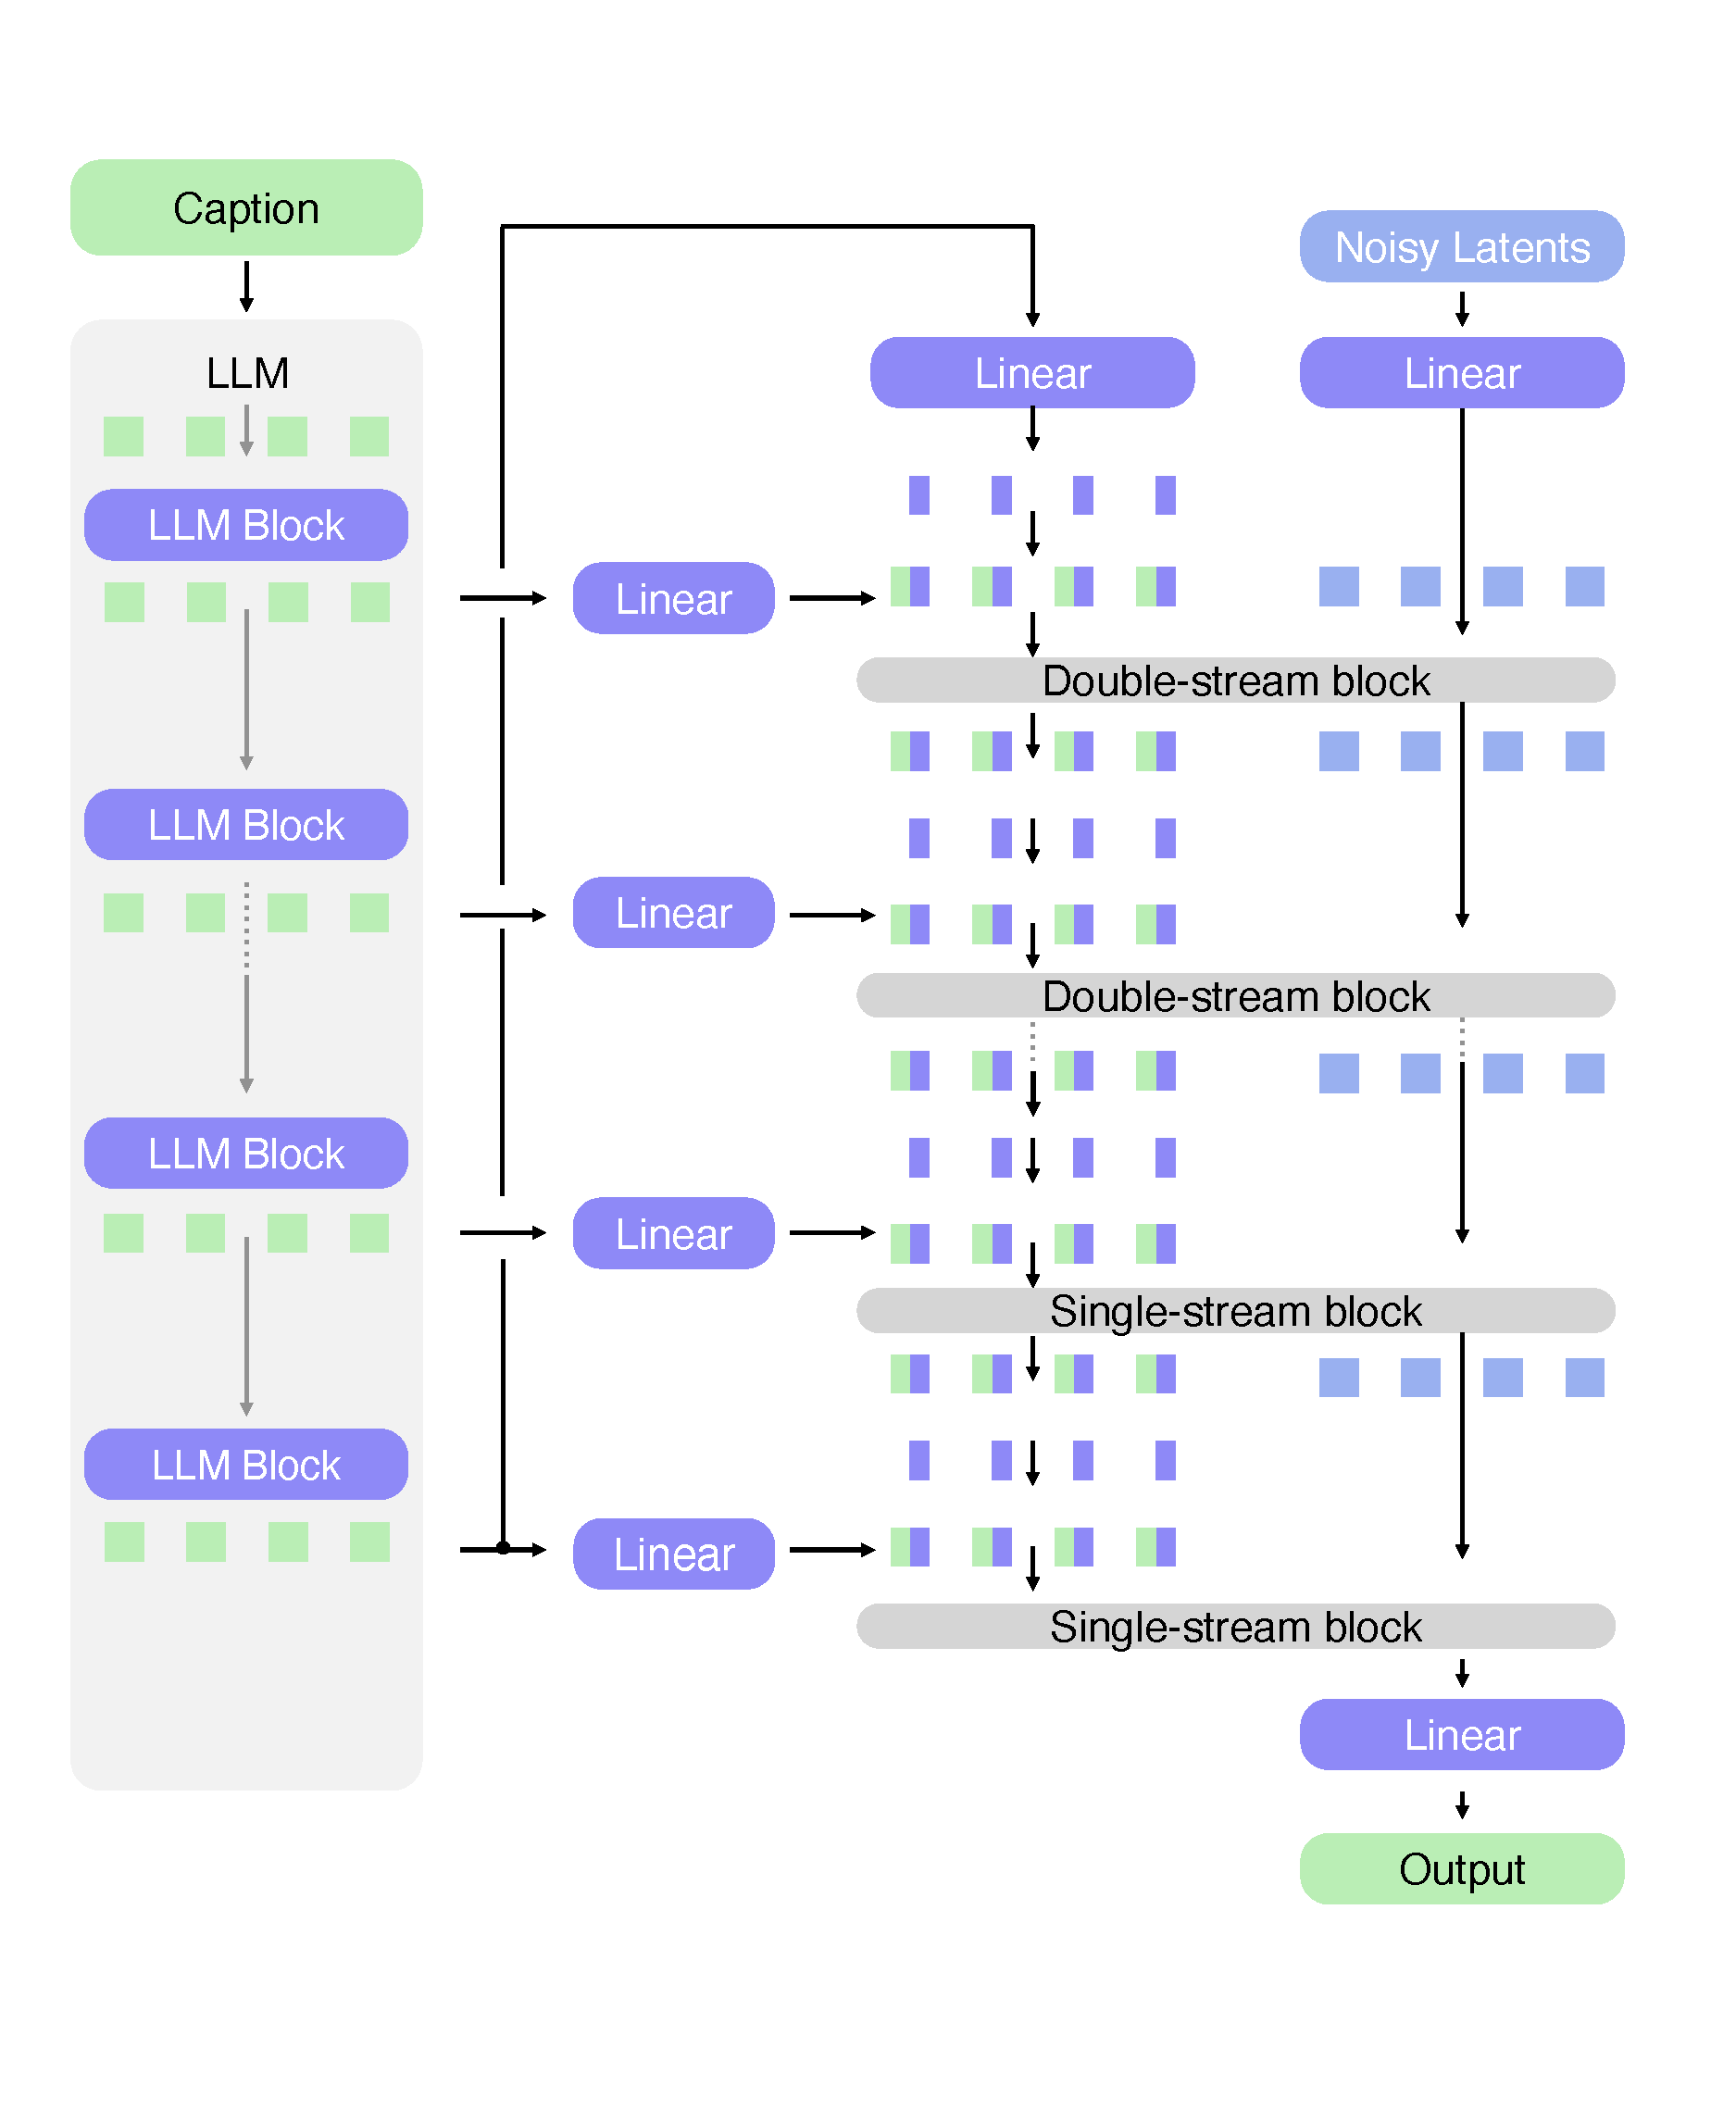
\includegraphics[width=\linewidth]{plots/model_figure2.pdf}
  \caption{\textbf{DimFusion architecture.} In each layer, the \textbf{\textcolor{textencoding}{text encoding}} is concatenated with the corresponding LLM \textbf{\textcolor{llmtokens}{hidden states}} along the embedding dimension. The resulting representation is then jointly processed with the \textbf{\textcolor{imagetokens}{noisy latents}} through bi-directional mixing in the Dual- and Single-stream blocks. After each block, the appended LLM hidden states are discarded, restoring the original text embedding dimension.}
  \label{fig:arch}
\end{figure}